\section{Special Case Analysis}

\subsection{Definitions}

\begin{frame}{Definitions}
  Its an empty frame to keep latex from compiling the movie!
  % \begin{columns}

  %   \column{0.5\textwidth}

  %     \begin{block}{Definition: 2D Stencil Interval Vertex Coloring (2DS-IVC)}<1->
  %       A problem where \( G \) is a \( 9 \)-pt \( 2D \) stencil, 
  %       composed of \( X \times Y \) vertices on a \( 2D \) grid such that two vertices \( (i, j) \) 
  %       and \( (i', j') \) are connected iff \( |i - i'| \leq 1 \) and \( |j - j'| \leq 1 \).
  %     \end{block}

  %     \null
  %     \centering
  %     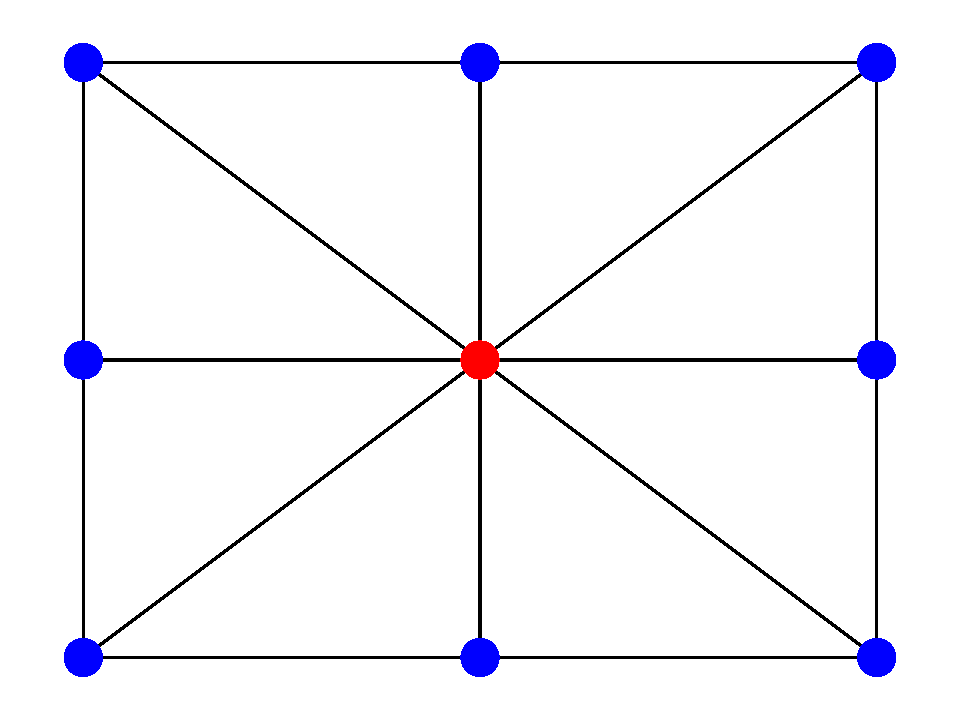
\includegraphics[width=0.5\textwidth]{figures/9pt_stencil_graph.pdf}<2->

  %     \null
  %     \null
  %     \null
  %     \null


  %   \column{0.5\textwidth}
  %     \begin{block}{Definition: 3D Stencil Interval Vertex Coloring (3DS-IVC)}<3->
  %       A problem where \( G \) is a 27-point \( 3D \) stencil, 
  %       composed of \(X \times Y \times Z\) vertices on a 3D grid such that two vertices 
  %       \( (i, j, k) \) and \( (i', j', k') \) are connected iff \( |i - i'| \leq 1 \), \( |j - j'| \leq 1 \), and
  %       \( |k - k'| \leq 1 \).
  %     \end{block}
  %     \centering
  %     \only<4->{%
  %       \animategraphics[loop,width=\textwidth, autoplay]{30}{figures/animation_27pt/output_}{0001}{180}
  %     }
  % \end{columns}
\end{frame}

% \begin{frame}{More Blocks}{theorem, proof}

  
%   \begin{theorem}
%     This is a theorem.
%   \end{theorem}
%   \begin{proof}
%     This is a proof.  Donec suscipit luctus lacus ut viverra. Proin molestie
%     eros tellus, vitae elementum nulla fringilla nec. Pellentesque facilisis,
%     elit ac egestas gravida, ante leo euismod velit, et suscipit est ex ut ex.
%   \end{proof}
% \end{frame}